\documentclass[../main.tex]{subfiles}

\begin{document}
	
\chapter{Розробка і тестування системи}
	
\section{Розробка  системи}
	
\subsection{Обґрунтування вибору засобів реалізації}

\textbf{Операційна система.}
Існує декілька найпоширеніших операційних систем для смартфонів, такі як Android, IOS та ін. Для розробки додатку за темою дипломної роботи було обрано операційну систему Android, тому що: 
\begin{itemize}[label={--}]
	\item вона має відкритий вихідний код;
	\item частка пристроїв на Android значно більша, ніж на інших операційних системах (див. рис. \ref{chart:market_share});
	\item абсолютно безкоштовна для розробки.
\end{itemize}

\begin{figure}[H]
	\centering
	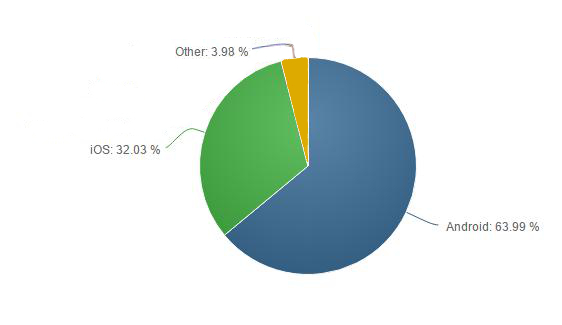
\includegraphics[width=1\textwidth]{market_share_2016}
	\caption{Частка пристроїв на різних ОС станом на 2016 рік}
	\label{chart:market_share}
\end{figure}

Також, було обрано мінімальну версію API для розробки додатку. Як видно з рис. \ref{chart:android_versions}, пристроїв під керуванням Android нижче версії API 19 досить мало, тому можна було б їх проігнорувати, та встановити її як мінімальну. Однак, для розроблюваного додатку для цього немає гострої необхідності, тому було обрано API версії 16 як мінімальну.\\

\begin{figure}[H]
	\centering
	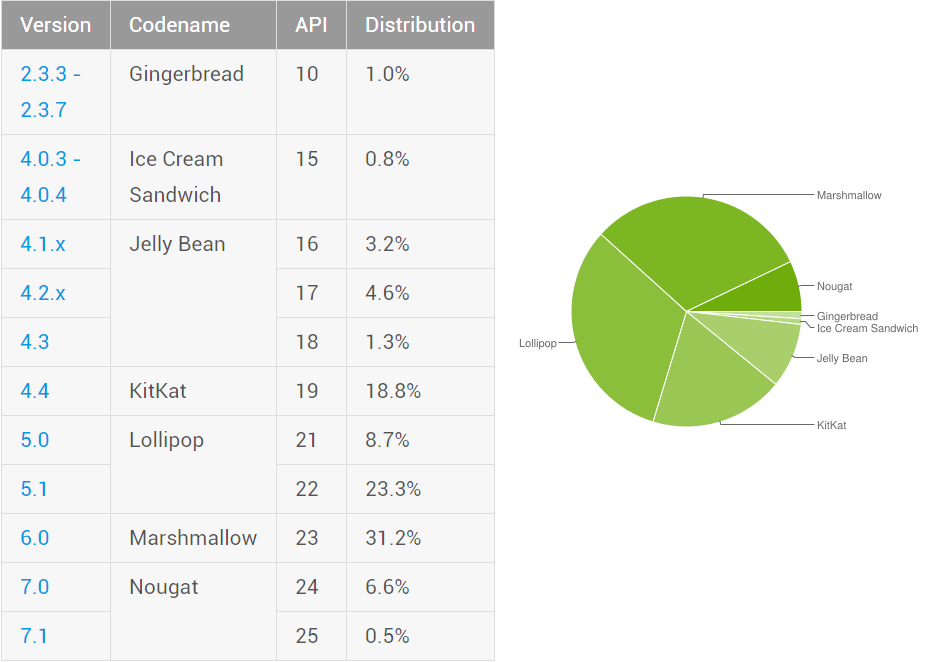
\includegraphics[width=1\textwidth]{android_versions}
	\caption{Відносна кількість пристроїв, що працюють під управлінням різних версій Android}
	\label{chart:android_versions}
\end{figure}

\textbf{Мова програмування.} 
В якості мови програмування для реалізації Android-щоденника було обрано мову Java. Ця мова повністю об'єктно-орієнтована. Всі сутності в Java є об'єктами, за виключенням основних (примітивних) типів: boolean, int, long, double і т.д. 

Розробниками Java був проведений фундаментальний аналіз програм на мові C++. В результаті цього аналізу вони вилучили можливість явного виділення і звільнення пам'яті. Наприклад, пам'ять в Java звільняється автоматично за допомогою механізму збору сміття (garbage collection), тому розробник застрахований від помилок, що виникають під час неправильного використання пам'яті. Однією з особливістей Java є відсутність множинного наслідування. Замість цього існує можливість імплементувати декілька інтерфейсів.

У тому числі, засоби для розробки під операційну систему Android написані на Java та більшість документації для Android містить приклади коду на цій мові.

\textbf{Середовище розробки.}
В якості середовища розробки було обрано Android Studio IDE, так як вона офіційна та постійно оновлюється. Серед функцій, що є в Android Studio, можна виділити такі:

\begin{enumerate}
	\item Розширений редактор макетів, що дозволяє працювати з компонентами користувацього інтерфейсу за допомогою перетягування їх на поле, що представляє екран пристрою. Також присутня функція попереднього перегляду макету при різних конфігураціях екрану.
	\item Збирання проектів основане на Gradle.
	\item Потужні інструменти для рефакторингу.
	\item Статичний аналізатор коду (Lint), що дозволяє знаходити проблеми продуктивності, несумісності версій та інших проблем.
	\item Різні види збірок та генерація декількох .apk файлів.
	\item Вбудований ProGuard (утиліта, призначена для оптимізації та обфускації Java коду), та утиліта для підпису додатків.
	\item Шаблони основних макетів та компонентів Android.
	\item Вбудована підтримка Google Cloud Platform, котра включає в себе інтеграцію з сервісами Google Cloud Messaging та App Engine.
	\item Підтримка останніх весрій Android SDK, в тому числі і Preview версій.
	\item З версії 2.1 підтримує оновлений компілятор Jack, також було покращено підтримку Java 8.
	\item Підтримка розробки додатків для Android Wear та Android TV.
\end{enumerate}

%TODO: add screenshots

\textbf{База даних.}
Для роботи з базою даних було вирішено використовувати сервіс Firebase. Він являє собою постачальника хмарних сервісів і додатків. Головний офіс знаходиться в Сан-Франциско, Каліфорнія. У 2011 році Andrew Lee і James Tamplin заснували Firebase і в квітні 2012 запустили хмарний сервіс. Основний напрямок Firebase -- хмарна noSQL база даних для real-time додатків (що працюють в режимі реального часу), яка надає API, що дозволяє розробникам зберігати та синхронізувати дані між декількома клієнтами. У жовтні 2014 року компанія була придбана Google, та у травні 2016 на конференції Google I/O було представлено значну кількість нових функцій.

Firebase надає real-time базу даних як сервіс, що в свою чергу має API для розробників, котра дозволяє синхронізувати дані додатку між клієнтами та зберігати їх у хмарі Firebase (див. рис. \ref{figure:firebase_workflow}). Компанія надає клієнтські бібліотеки, які дозволяють інтеграцію з Android, IOS, JavaScript, Java, Objective-C, Swift та Node.js додатками. Робота безпосередньо з базою даних реалізована через REST сервіси для деяких JavaScript фрейморків, таких як AngularJS, React, Ember.js і Backbone.js. REST API використовує протокол Server-Sent Events (SSE). Розробники, що використовують цю БД можуть захистити свої дані за допомогою встановлення правил безпеки на стороні серверу \cite{firebase_secure}.

\begin{figure}[H]
	\centering
	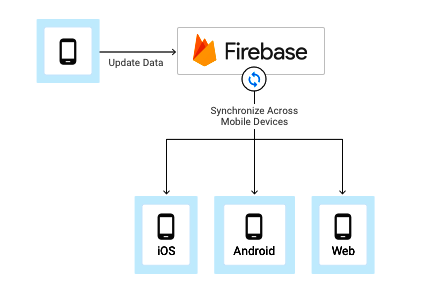
\includegraphics[width=0.8\textwidth]{firebase_workflow}
	\caption{Принцип роботи real-time бази даних Firebase}
	\label{figure:firebase_workflow}
\end{figure}

Основні можливості бази даних Firebase:
\begin{enumerate}
	\item \textit{Миттєва синхронізація.} Замість типових запитів HTTP, real-time база даних Firebase використовує синхронізацію даних -- кожен раз, коли дані змінюються, будь-який підключений пристрій отримує ці оновлення миттєво.
	\item \textit{Автономність.} Firebase додатки залишаються працездатним навіть в автономному режимі, так як Firebase SDK зберігає дані на диск. Після того, як підключення буде відновлено, пристрій клієнту отримає всі зміни, що було пропущено, та синхронізується з поточним станом сервера.
	\item \textit{Зручний доступ з пристроїв клієнтів.} Доступ до бази даних Firebase можна отримати безпосередньо з мобільного пристрою або веб-браузеру, немає необхідності для серверу. Безпека та перевірка даних доступні через правила безпеки для бази даних Firebase -- основані на виразах правила, котрі виконуються, коли дані зчитуються або записуються.
\end{enumerate}

База даних Firebase являє собою noSQL базу і має різні оптимізації та функціональні можливості в порівнянні з реляційною базою. API бази Firebase побудована так, щоб дозволити тільки операції, котрі можуть бути виконані швидко. Це дозволяє будувати чудові real-time рішення, що можуть служити мільйонам користувачів без шкоди для гнучкості. Через це, важливо думати про те, як користувачі повинні отримувати доступ до даних, а потім структурувати їх відповідним чином.

Для збереження файлів Firebase надає зручний сервіс Cloud Storage -- потужний, простий та рентабельний сервіс для збереження об'єктів. Firebase SDK для хмарного збереження даних додає безпеки до процесу вивантаження та завантаження файлів для Firebase додатків, незалежно від якості мережі. Також, є можливість використовувати цю SDK для зберігання зображень, аудіо, відео або іншого контенту, що створюють користувачі. На сервері, можна використовувати Google Cloud Storage, щоб отримати доступ до тих же файлів.

Основні можливості хмарного сховища Firebase:
\begin{enumerate}
	\item \textit{Надійні операції.} Firebase SDK для хмарного сховища дозволяє вивантаження та завантаження незалежно від якості мережі. Вивантаження та завантаження надійні, тобто вони перезапускаються там, де зупинилися, зберігаючи час користувачів і пропускну здатність.
	\item \textit{Безпечність.} Також, ця SDK інтегрована з Firebase аутентифікацією, щоб забезпечити просту та інтуїтивно зрозумілу аутентифікацію для розробників, котрі можуть використовувати декларативну модель безпеки, щоб дозволити доступ на основі ім'я файлу, розміру, типу контенту та інших метаданих.
	\item \textit{Висока масштабованість.} Хмарне сховище Firebase побудоване для великих масштабів, для додатків, що розвиваються від прототипу до виробництва використовучи такі ж інфраструктури, як Spotify чи Google Photos.
\end{enumerate}

Розробники використовують Firebase SDK хмарного сховища для вивантаження та завантаження файлів безпосередньо від клієнтів. Збережені в хмарному сховищі Firebase файли доступні як через Firebase, так і через Google Cloud. Це дозволяє завантажувати файли з мобільних клієнтів через Firebase SDK і виконувати обробку на стороні сервера, таку як фільтрація зображень або перекодування відео, за допомогою Google Cloud Platform. Хмарне сховище масштабується автоматично, тому немає ніякої необхідності переходити до інший постачальників.

%TODO: add info about Firebase Auth https://firebase.google.com/docs/auth/

Також, Firebase має безліч інших інструментів для розробників (див. рис. \ref{figure:firebase_tools}), якими користуються такі компанії, як The New York Times, Shazam, duolingo, Alibaba.com та інші \cite{firebase}.

%TODO: add info about Goole Location, Maps, Places

\begin{figure}[H]
	\centering
	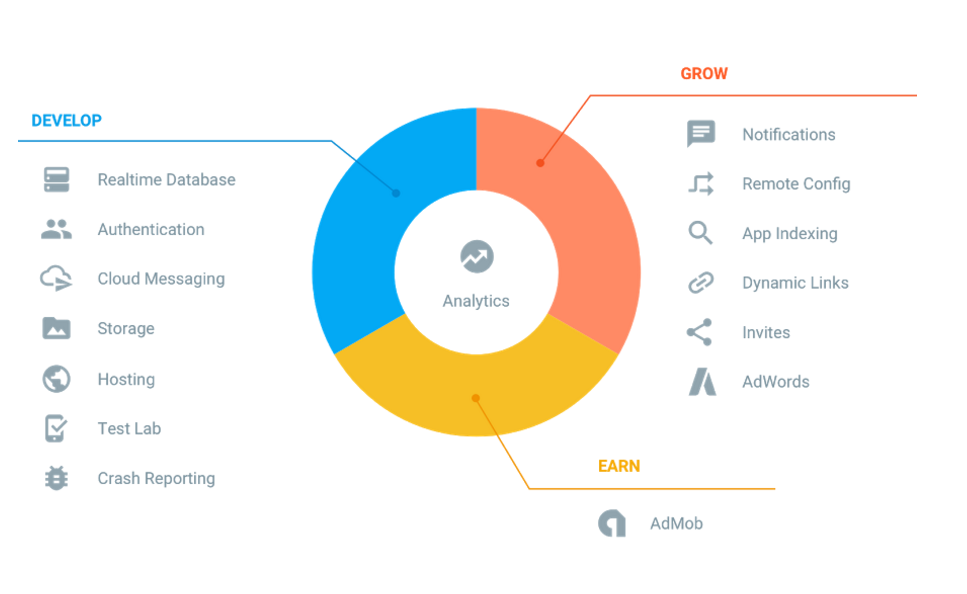
\includegraphics[width=1\textwidth]{firebase_tools}
	\caption{Набір інструментів Firebase}
	\label{figure:firebase_tools}
\end{figure}

\subsection{Опис структурної (функціональної) схеми}

%TODO

\subsection{Опис логічної схеми}
Для того, щоб користувач мав змогу користуватися додатком, йому потрібно пройти авторизацію використовуючи обліковий запис Google. Користувач може обрати вже існуючий, або додати новий акаунт. Після вибору акаунту проходить авторизація до серверу Firebase, після чого, якщо вона прошла успішно, користувач може починати роботу з додатком. Якщо ж вибір акаунту чи авторизація до Firebase пройшли невдало, користувачу потрібно повторити спробу. Блок-схема процесу авторизації користувача зображена на рис. \ref{diagram:login}.

\begin{figure}[H]
	\centering
	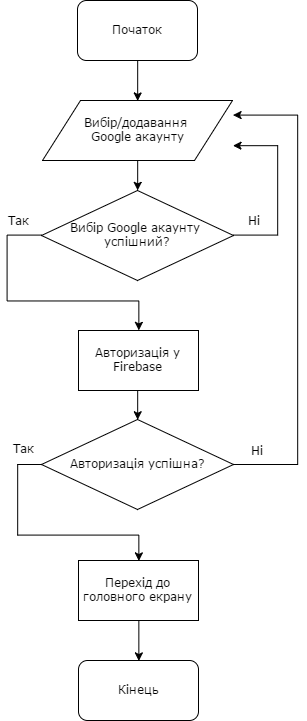
\includegraphics[height=1\textwidth]{login_diagram}
	\caption{Блок-схема авторизації користувача}
	\label{diagram:login}
\end{figure}

Для запису треку переміщень повинна бути активна подорож. Якщо активної подорожі немає, кнопка запису трека стає неактивною. Тому, для того щоб почати запис, користувач повинен спочатку зробити активною будь-яку подорож. Блок-схему для початку запису трека переміщень подано на рис. \ref{diagram:start_tracking}.

\begin{figure}[H]
	\centering
	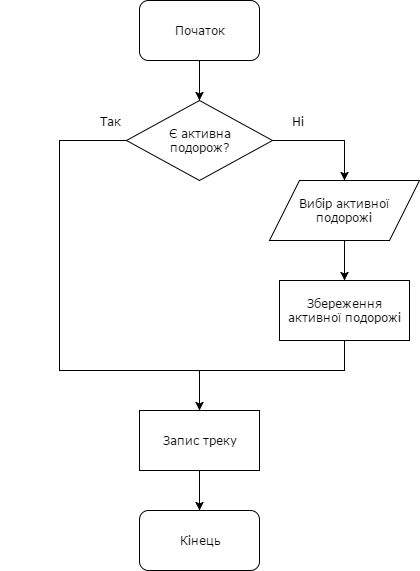
\includegraphics[height=1\textwidth]{record_track_diagram}
	\caption{Блок-схема старту запису трека переміщень}
	\label{diagram:start_tracking}
\end{figure}

Для створення подорожі користувачу потрібно ввести її назву та опис. Назва є обов'язковим полем, тому, якщо користувач спробує зберегти подорож з порожньою назвою, йому буде відмовлено та запропоновано ввести назву для цієї подорожі. Блок-схема створення та редагування подорожі зображена на рис. \ref{diagram:travel_creation}.

\begin{figure}[H]
	\centering
	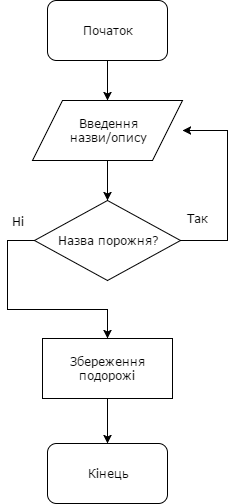
\includegraphics[height=1\textwidth]{travel_creation_diagram}
	\caption{Блок-схема створення подорожі}
	\label{diagram:travel_creation}
\end{figure}

\subsection{Розробка бази даних}
При розробці бази даних було виділено такі основні сутності: \textit{User}~(Користувач), \textit{Travel}~(Подорож), \textit{Diary}~(Щоденник) та \textit{Reminder}~(Планувальник). Користувач може мати безліч подорожей, котрі в свою чергу можуть містити будь-яку кількість записів щоденника та планувальника. Додатково, було створено сутності для інформації про погоду та адресу, для того, щоб зберігати її для запису щоденника. Для збереження фото служить сутність \textit{Photo}, а сутність \textit{Location} потрібна для збереження координат. Для нагадувань за місцем для планувальника існує сутність \textit{WayPoint}, вона містить назву місця (яка також використовується для відображення на карті), та  координати, для яких встановлене нагадування. Для запису трека переміщень створено сутність \textit{Track}, яка містить список координат. Схема бази даних зображена на рис. \ref{diagram:database}.

\begin{figure}[H]
	\centering
	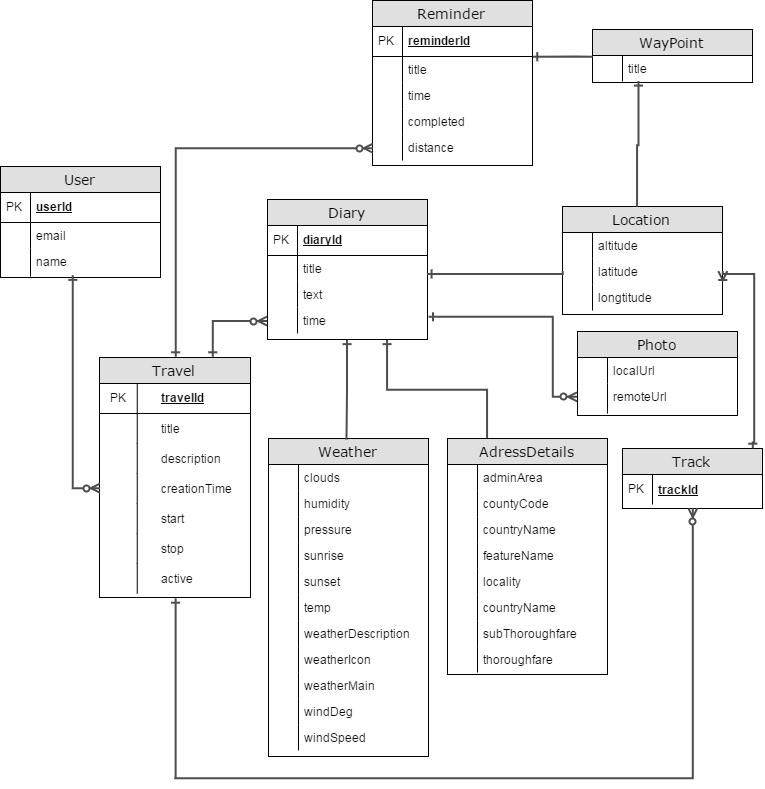
\includegraphics[width=0.9\textwidth]{database}
	\caption{Схема бази даних}
	\label{diagram:database}
\end{figure}

За допомогою консолі розробника Firebase для бази даних було встановлено такі правила безпеки:
\begin{center}
	\textit{".write": "auth !== null \&\& auth.uid === \$uid"}\\
	\textit{".read": "auth !== null \&\& auth.uid === \$uid"},
\end{center}

які означають, що читати та записувати дані зможуть лише авторизовані коритсувачі та лише для своєї гілки (для якої ключ користувача дорівнює ключу авторизованого користувача).

\subsection{Розробка інтерфейсу користувача}
Інтерфейс потрібний для взаємодії користувача з додатком. Ефективність інтерфейсу визначається здатністю передбачити вимоги користувачів, які будуть виникати при використанні додатку. 

Для розробки інтерфейсу Android-щоденника використовувалися правила матеріального дизайну. Material Design (Матеріальний дизайн) -- дизайн програмного забезпечення та додатків операційної системи Android від компанії Google. Вперше представлений на конференції Google I/O 25 червня 2014 року.  Ідея дизайну полягає в інтерфейсі, поведінка і вигляд якого наслідують правила поведінки і вигляду паперових карток в реальному житті. 

Material Design грунтується на чотирьох основних принципах:

\begin{enumerate}
	\item \textit{Тактильні поверхні.} У цьому дизайні інтерфейс складається з відчутних шарів. Ці шари розташовані на різній висоті і відкидають тіні один на одного, що допомагає користувачам краще розуміти анатомію інтерфейсу і принцип взаємодії з ним.
	\item \textit{Поліграфічний дизайн.} Використовується підхід з традиційного графічного дизайну (журнального, плакатного і т. д.).
	\item \textit{Осмислена анімація.} У реальному світі предмети не виникають нізвідки і не зникають в нікуди, тому в Material Design потрібно за допомогою анімацій давати користувачам підказки про роботу інтерфейсу.
	\item \textit{Адаптивний дизайн.} Потрібно застосовувати попередні три концепції так, щоб на різних пристроях з різною роздільною здатністю та розмірами екранів все виглядало як задумано.
\end{enumerate}

Оскільки головними елементами щоденника для мандрівників є мандрівки, то на головному екрані розмістився список з ними. В якості елементів списку виступають картки, що містять назву, дати початку та кінця подорожі й зображення на фоні. Також, для активної подорожі присутній індикатор. В правому нижньому кутку розміщено кнопку, що є компонентом матеріального дизайну та називається \textit{Floating Action Button}. Зазвичай вона використовується для основних дій. На даному екрані такою дією є створення нової подорожі. Головний екран зі списком подорожей зображено на рис. \ref{figure:main_screen}.

\begin{figure}[H]
	\centering
	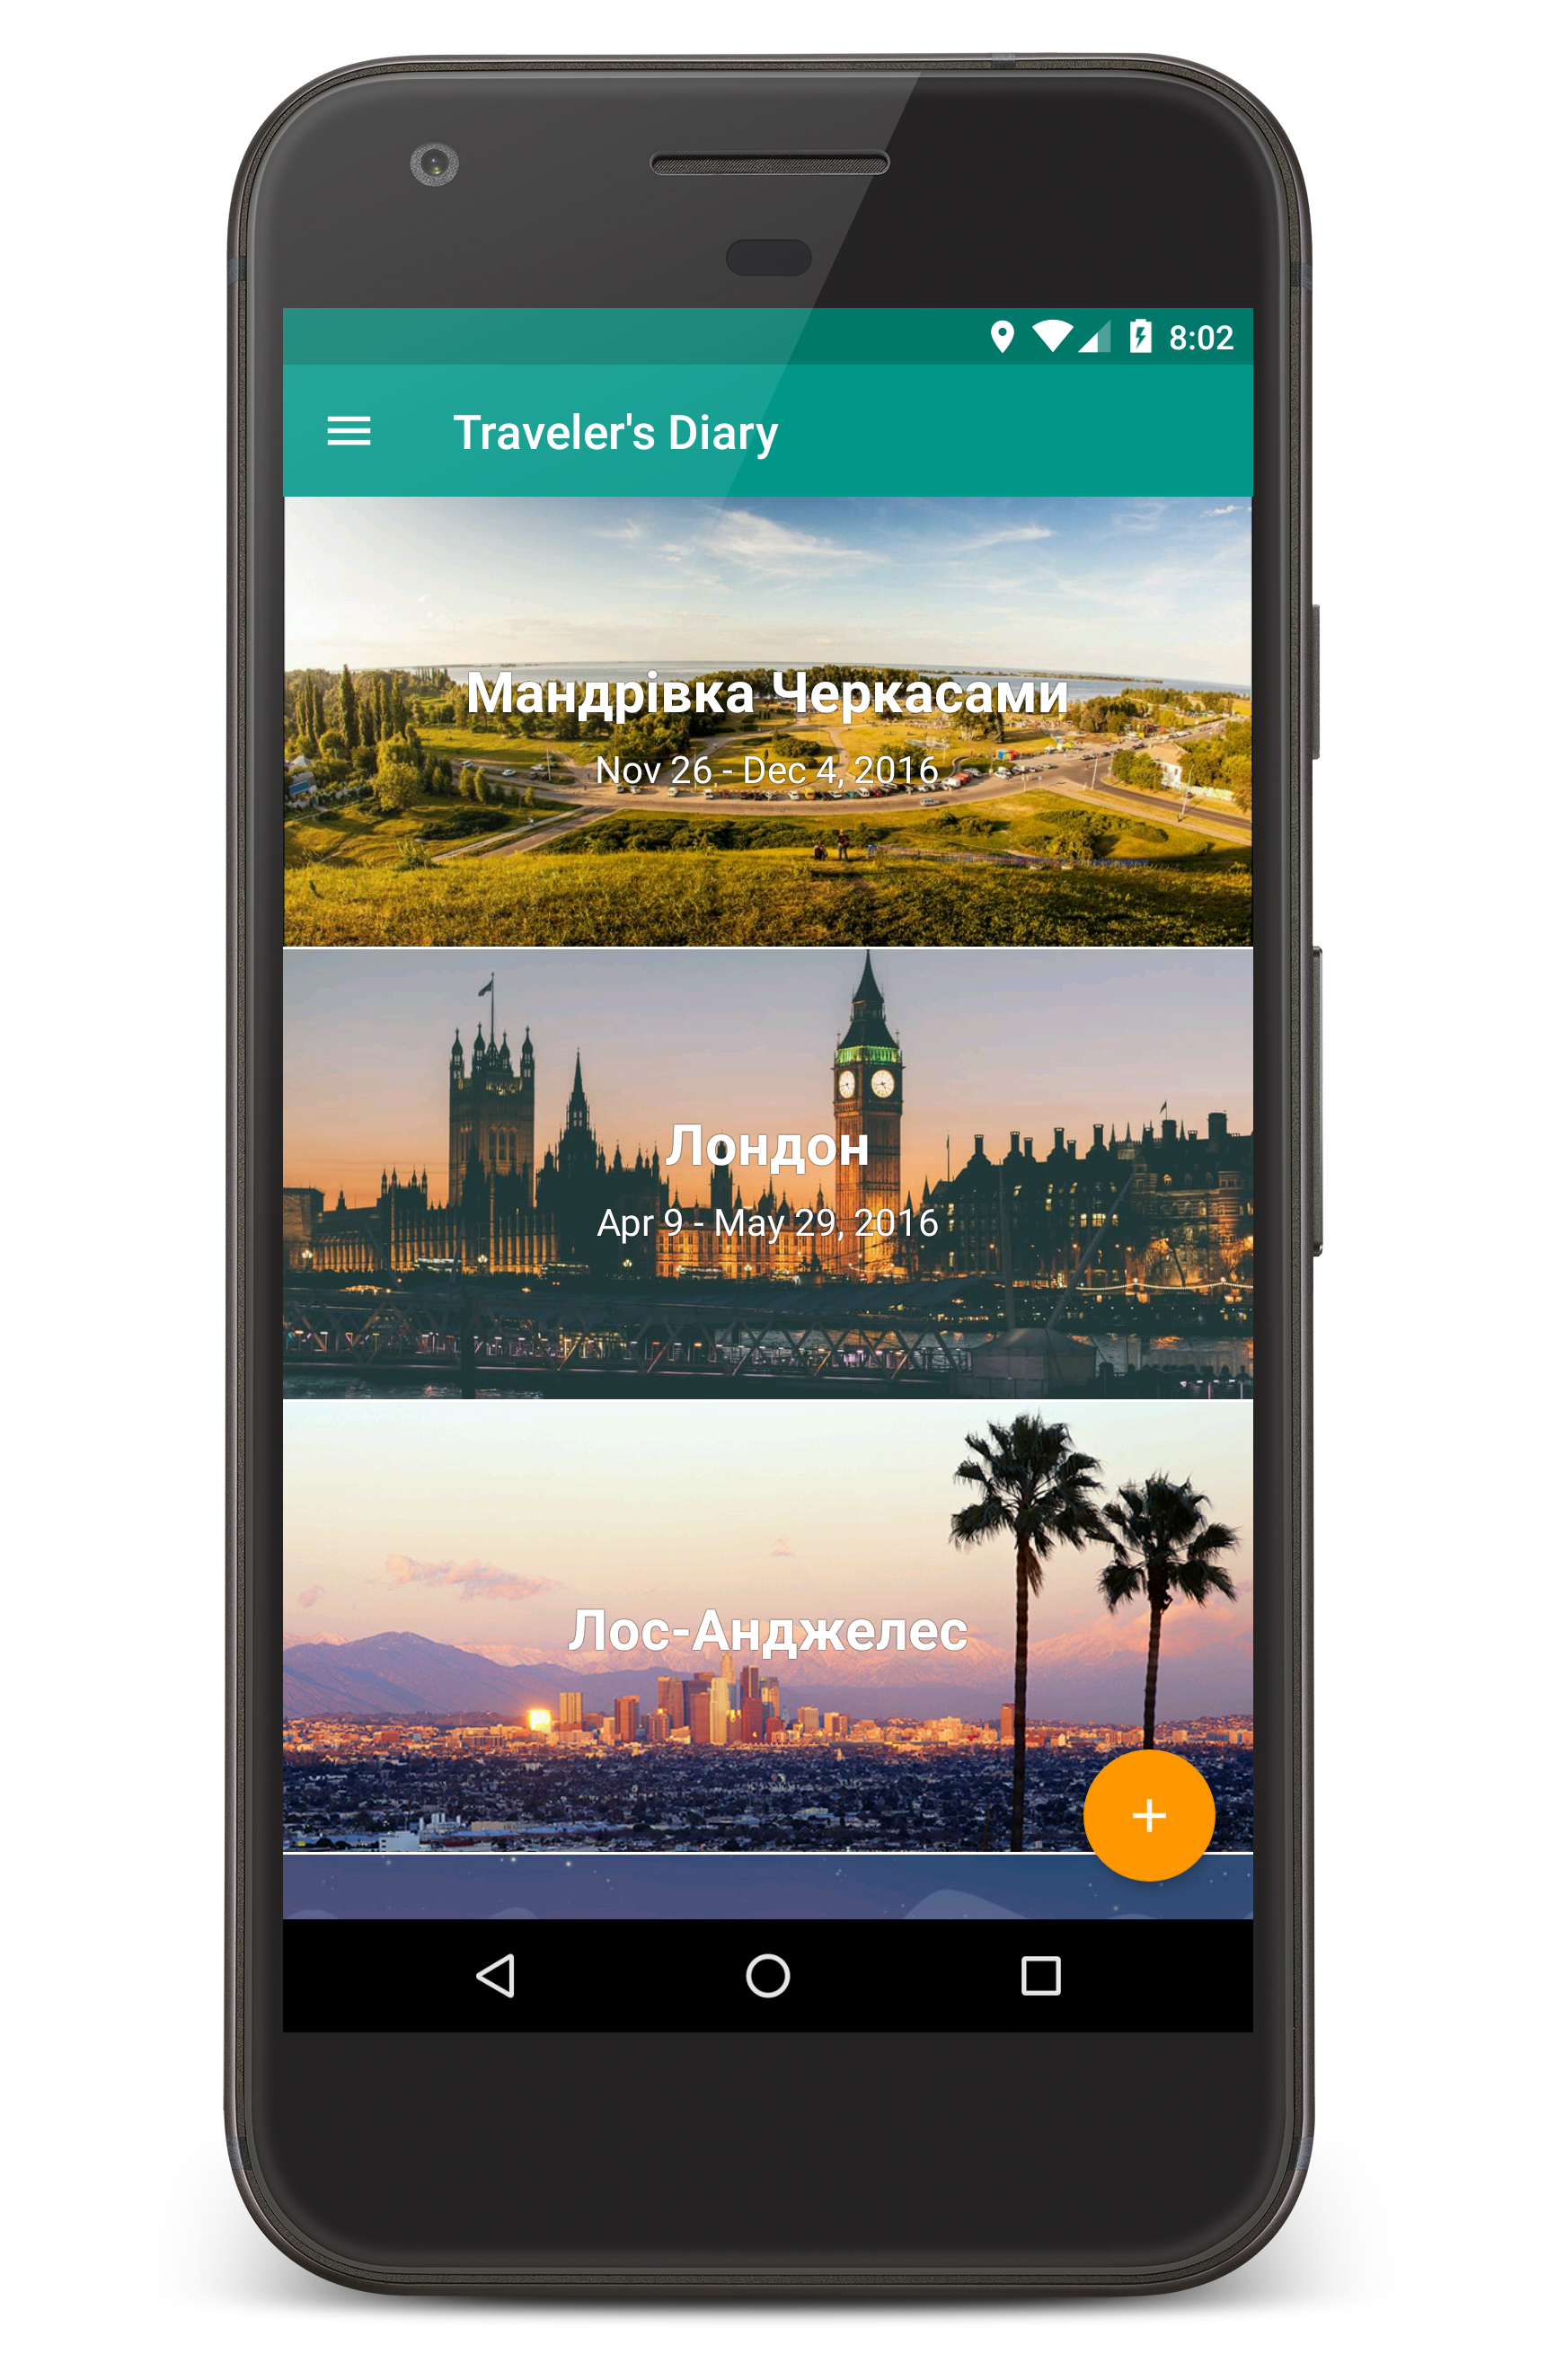
\includegraphics[width=0.6\textwidth]{main_screen}
	\caption{Головний екран додатку зі списком подорожей}
	\label{figure:main_screen}
\end{figure}

Для відображення 

\begin{figure}[H]
	\centering
	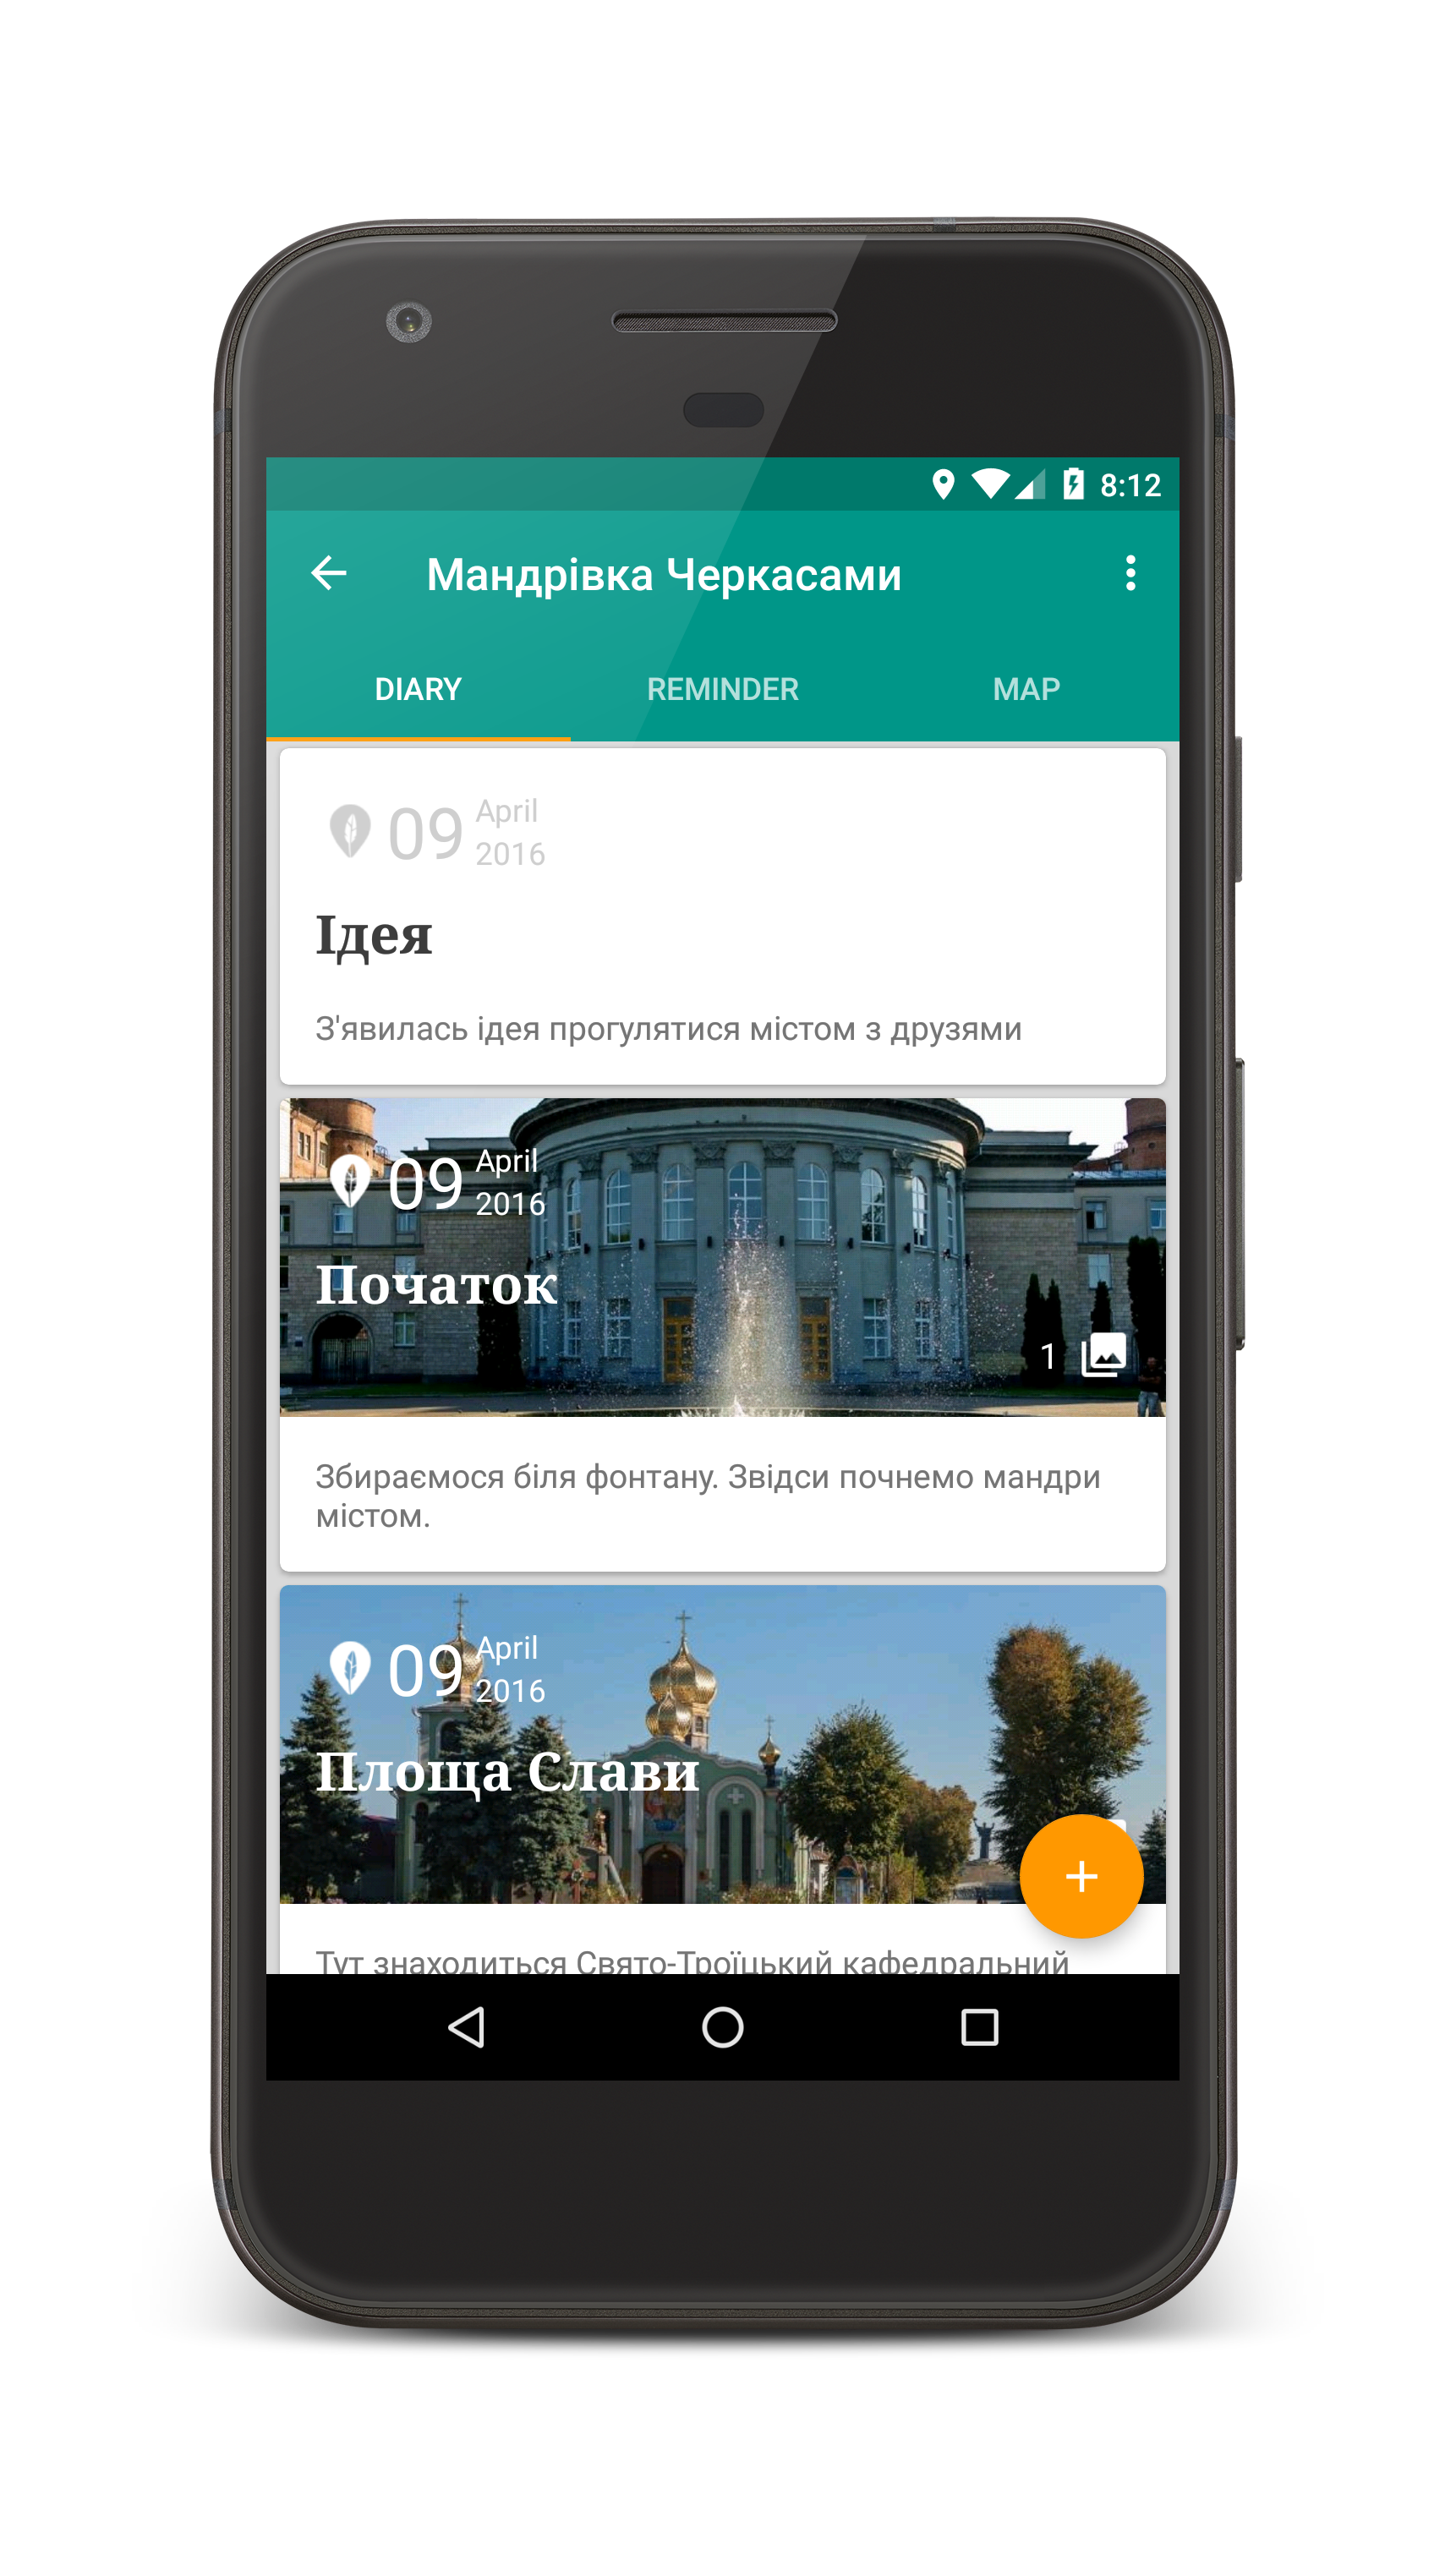
\includegraphics[width=0.6\textwidth]{diarylist_screen}
	\caption{Diary list screen}
	\label{figure:diary_list_screen}
\end{figure}

\begin{figure}[H]
	\centering
	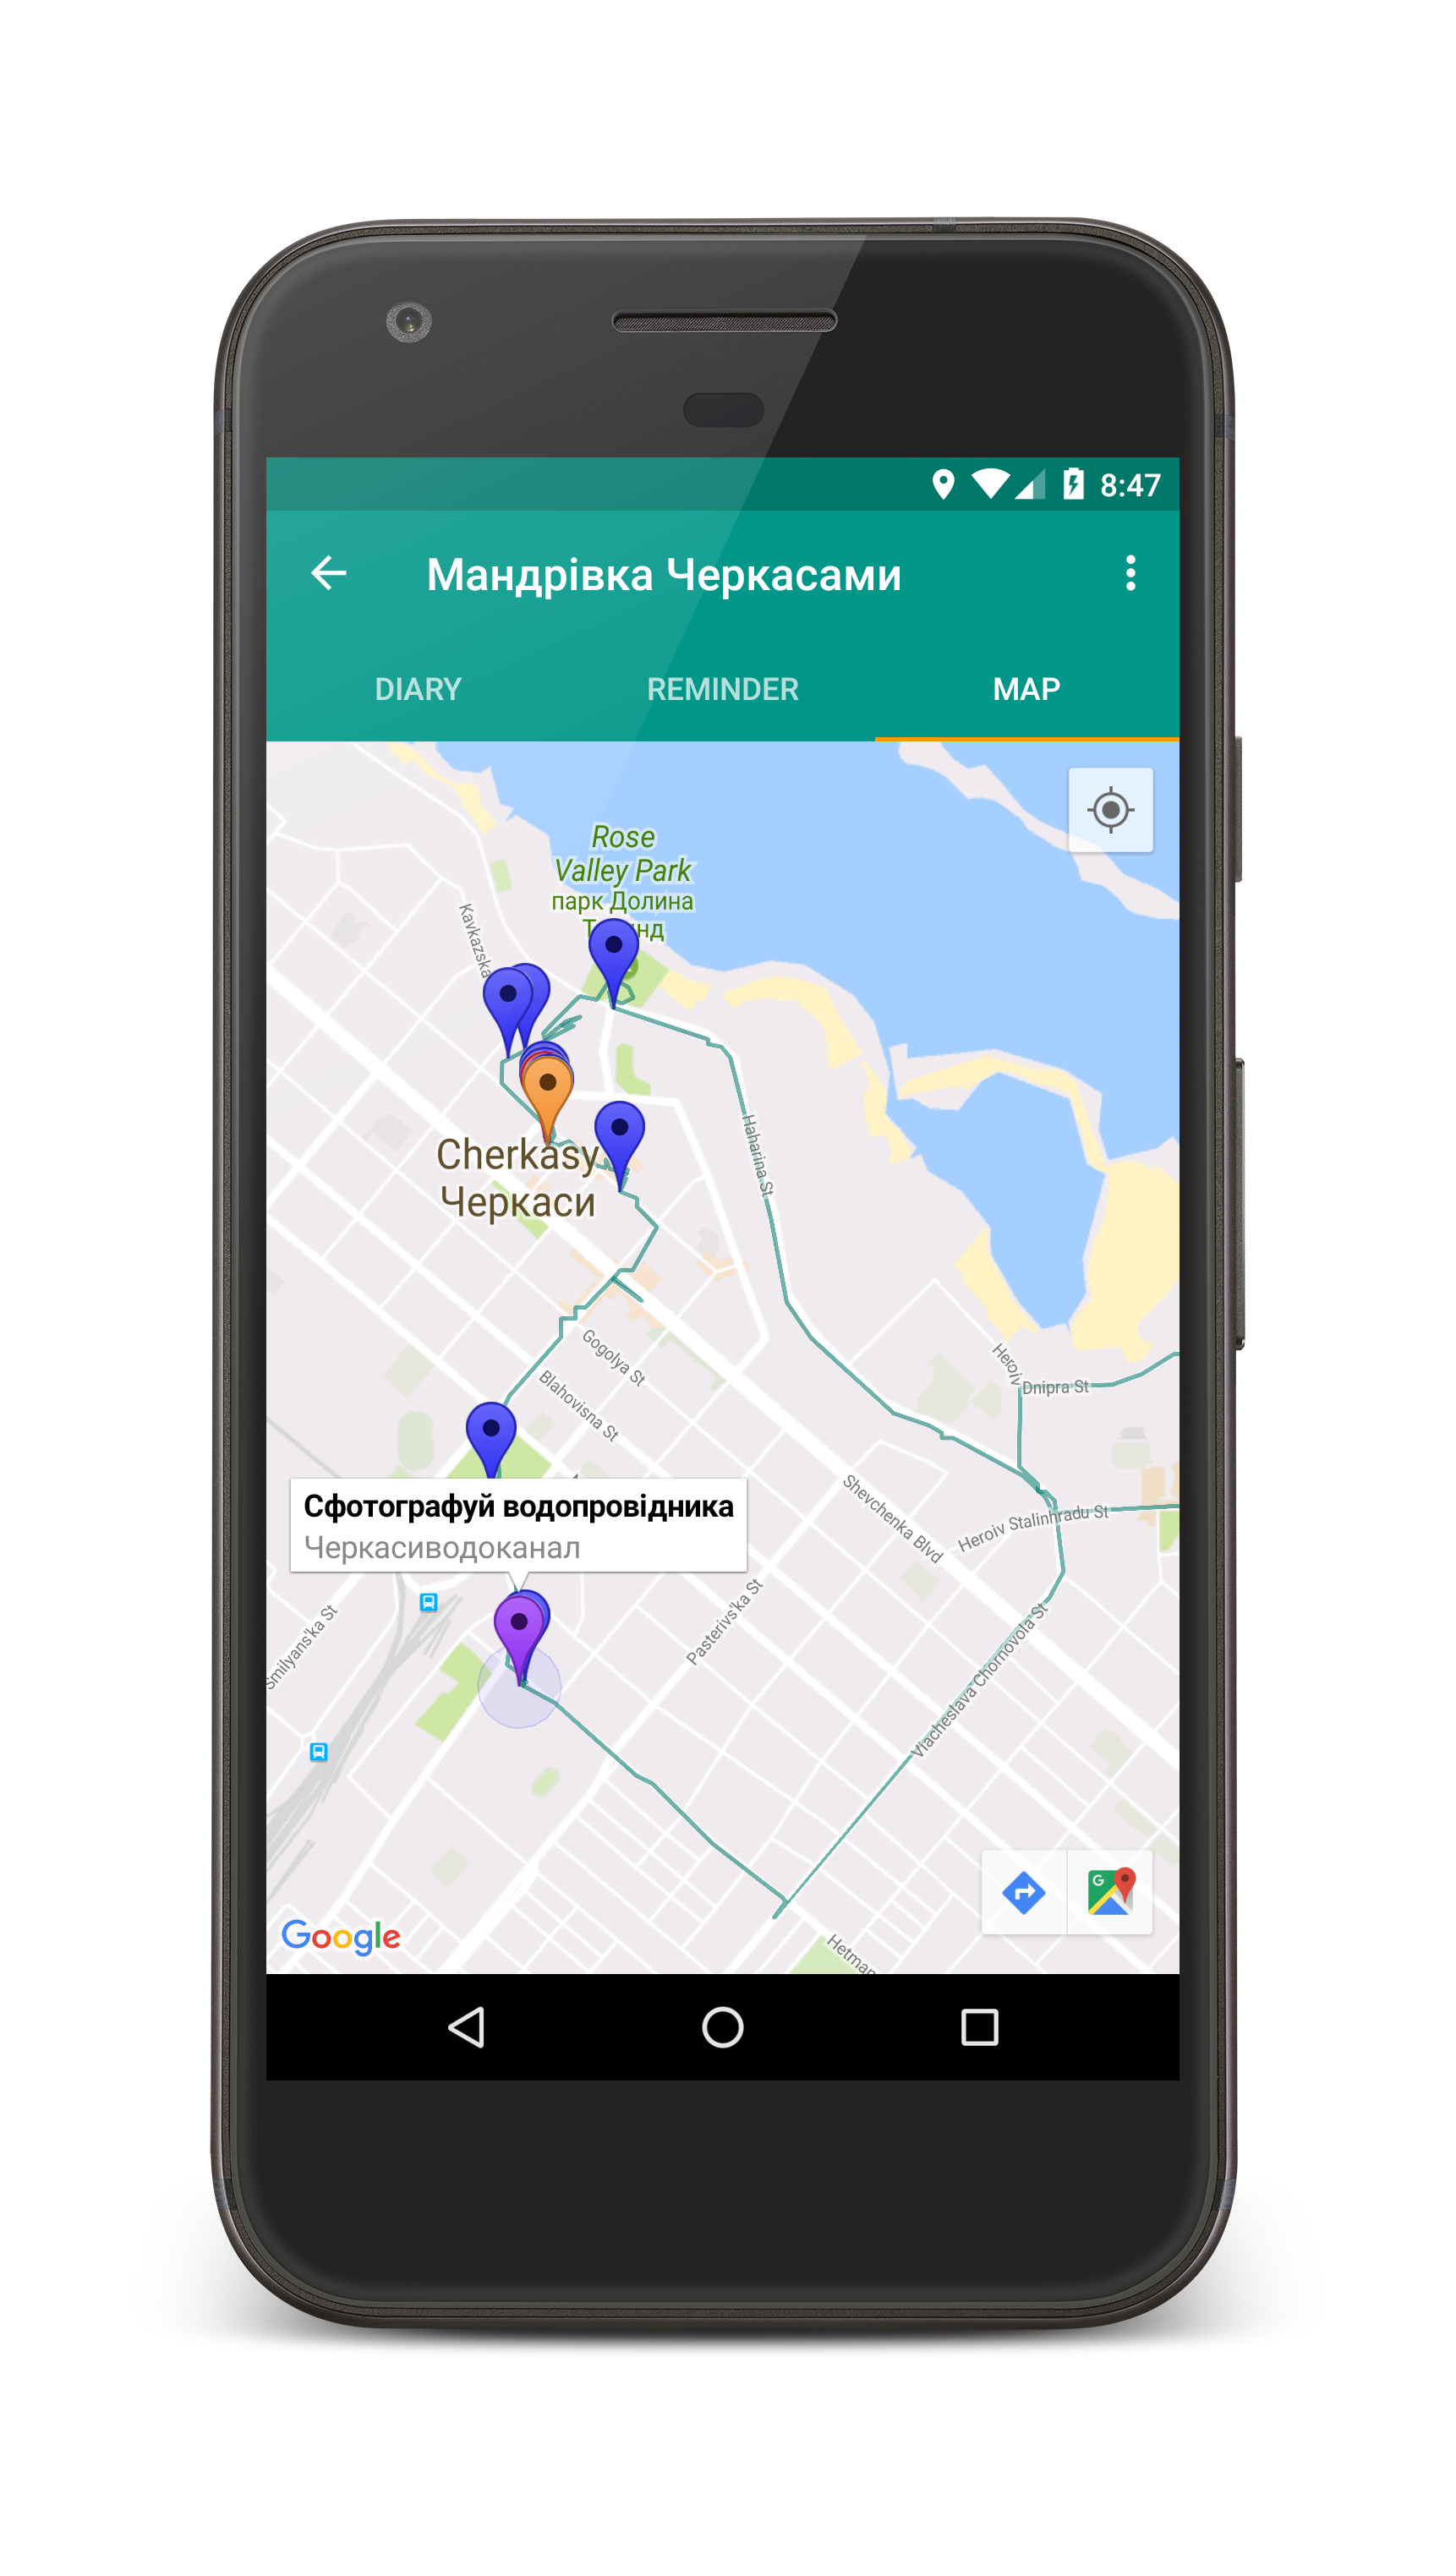
\includegraphics[width=0.6\textwidth]{map_screen}
	\caption{Map screen}
	\label{figure:map_screen}
\end{figure}

\subsection{Опис розробки програмних компонентів}

\section{Тестування інформаційної системи}

%TODO: write about db secure rules and access simulator

\section{Висновки}

% TODO: Висновки до розділу (не більш 1-2 сторінки). Розмір одного висновку приблизно – один абзац (5-7 рядків).
	
\end{document}